\documentclass[dvipdfmx]{jarticle}
\pagestyle{empty}
\usepackage{tikz}
\usepackage{fancyvrb}
\begin{document}
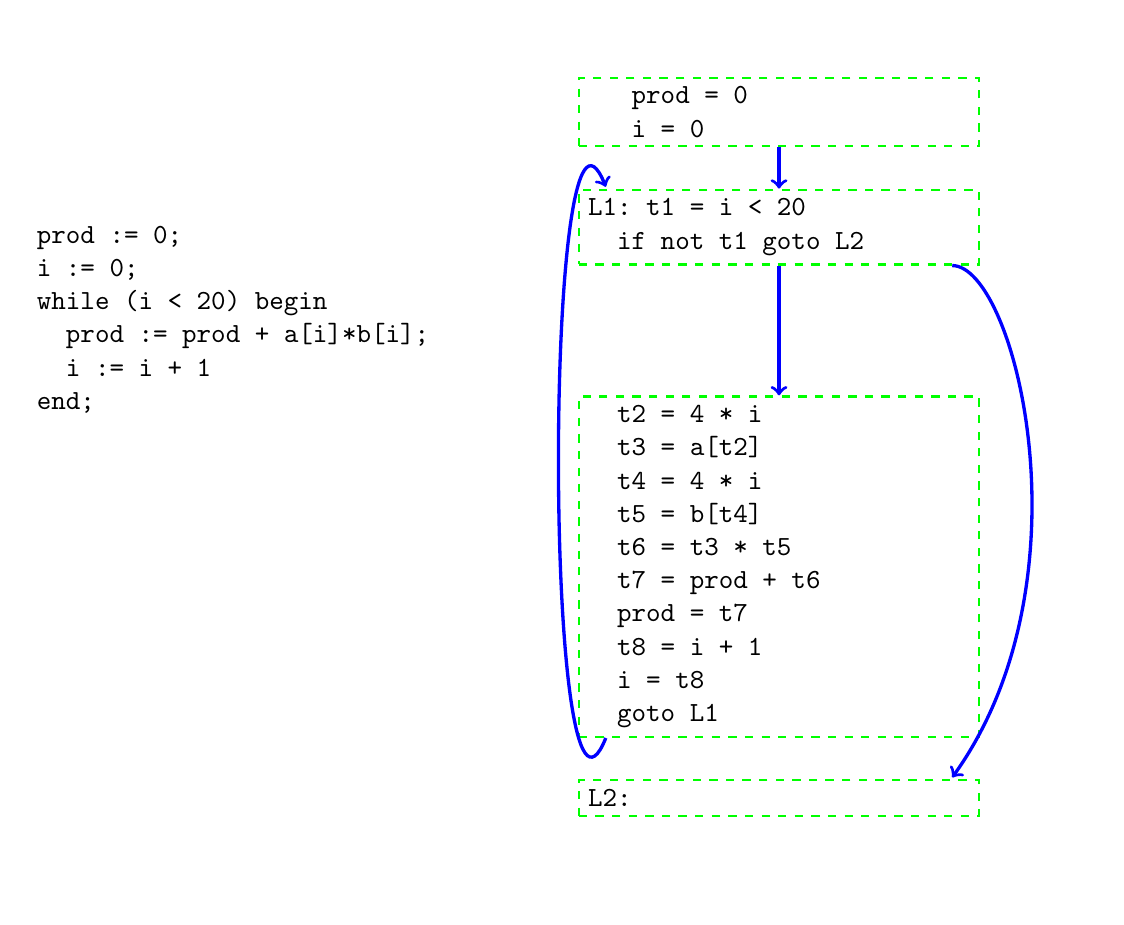
\begin{tikzpicture}

\node[above] (M) at (0,5) {
\begin{minipage}{.4\textwidth}
  \begin{Verbatim}
prod := 0;
i := 0;
while (i < 20) begin
  prod := prod + a[i]*b[i];
  i := i + 1
end;
  \end{Verbatim}
\end{minipage}
};

 \node[rectangle, draw=green, thick, dashed, above] (N0) at (7,8.5) {
 \begin{minipage}{.4\textwidth}
  \begin{Verbatim}
   prod = 0
   i = 0
  \end{Verbatim}
 \end{minipage}
 };

 \node[rectangle, draw=green, thick, dashed, above] (N1) at (7,7) {
 \begin{minipage}{.4\textwidth}
  \begin{Verbatim}
L1: t1 = i < 20 
  if not t1 goto L2
  \end{Verbatim}
 \end{minipage}
 };
 \node[rectangle, draw=green, thick, dashed, above] (N2) at (7,1) {
 \begin{minipage}{.4\textwidth}
  \begin{Verbatim}
  t2 = 4 * i
  t3 = a[t2]
  t4 = 4 * i
  t5 = b[t4]
  t6 = t3 * t5
  t7 = prod + t6
  prod = t7
  t8 = i + 1
  i = t8
  goto L1
  \end{Verbatim}
 \end{minipage}
};
 \node[rectangle, draw=green, thick, dashed, above] (N3) at (7,0) {
 \begin{minipage}{.4\textwidth}
  \begin{Verbatim}
L2:
  \end{Verbatim}
 \end{minipage}
};

\draw[->,very thick, blue]  (N0) -- (N1);
\draw[->,very thick, blue]  (N1) -- (N2);
\draw[->,very thick, blue]  (4.8,1) .. controls (4,-1) and (4,10) .. (4.8,8);
\draw[->,very thick, blue] (9.2,7) .. controls (10,7) and (11,3) .. (9.2,0.5);
\end{tikzpicture}
\end{document}
